\documentclass[11pt]{extarticle}
\usepackage[tmargin=1in,bmargin=1in,lmargin=1in,rmargin=1in]{geometry}
\usepackage[utf8]{inputenc}
\usepackage{tikz}
\usepackage{graphicx}
\usepackage{float}
\usepackage{setspace}
\usepackage{tabularx}
\usepackage[utf8]{inputenc}
\usepackage{caption}
\usepackage{subcaption}
\usepackage{framed}
\usepackage{enumitem}
\usepackage{amsmath}
\usepackage{mathpazo}
\usepackage{ragged2e}
\usepackage{titlesec}
\usepackage{framed}
\usepackage{color}   %May be necessary if you want to color links
\usepackage{hyperref}
\usepackage{footnotebackref}
\usepackage{listings}
\usepackage{xcolor}
\usepackage{fancyhdr}
\usepackage{lastpage}
\usepackage{lscape}

\hypersetup{
    colorlinks=true, %set true if you want colored links
    linktoc=section,     %set to all if you want both sections and subsections linked
    linkcolor=black,  %choose some color if you want links to stand out
}

\fancypagestyle{myheadings}
{
    \fancyhf{}
    \renewcommand{\footrulewidth}{0pt}
    \renewcommand{\headrulewidth}{0pt}
    \cfoot{Page \thepage\ of \pageref*{LastPage}}    
}

\fancypagestyle{plain}
{
    \fancyhf{}
    \chead{\small Delivery 03}
    \lhead{\small CS 353}
    \rhead{\small Spring 2022}
    % \renewcommand{\footrulewidth}{0.5pt}
    \renewcommand{\headrulewidth}{0.5pt}
    \cfoot{Page \thepage\ of \pageref*{LastPage}}    
}

\definecolor{mGreen}{rgb}{0,0.6,0}
\definecolor{mGray}{rgb}{0.5,0.5,0.5}
\definecolor{mPurple}{rgb}{0.58,0,0.82}
\definecolor{backgroundColour}{rgb}{0.95,0.95,0.92}

\lstdefinestyle{CStyle}{
    backgroundcolor=\color{backgroundColour},
    % backgroundcolor = \color{white},   
    commentstyle=\color{mGreen},
    keywordstyle=\color{magenta},
    numberstyle=\tiny\color{mGray},
    stringstyle=\color{mPurple},
    basicstyle=\footnotesize\bfseries\fontfamily{cmtt}\selectfont,
    breakatwhitespace=false,         
    breaklines=true,                 
    captionpos=b,                    
    keepspaces=true,                 
    numbers=left,                    
    numbersep=5pt,                  
    showspaces=false,                
    showstringspaces=false,
    showtabs=false,                  
    tabsize=2,
    frame = single,
    language=C
}

\title{\textbf{Project Delivery 03}}
\author{Aliza Rafique (05986); Asad Tariq (05439); Fahad Shaikh (05452); Faiz Haseeb (06224)}
\date{$8^{th}$ March 2022}


% Set formats for each heading level
\titleformat*{\section}{\Large\bfseries\fontfamily{phv}\selectfont}
\titleformat*{\subsection}{\large\bfseries\fontfamily{phv}\selectfont}
\titleformat*{\subsubsection}{\itshape\subsubsectionfont}

\providecommand\phantomsection{}

\doublespacing
\begin{document}
\begin{titlepage}
\thispagestyle{empty}
\begin{center}

\includegraphics[scale=0.40]{Figures/HU-LOGO--01.jpg}
\line(1,0){400}\\
[2mm]
\fontfamily{phv}\selectfont
\textbf{Project Proposal}\\
\line(2,0){250}\\
[0.5cm]
Submitted By\\
Aliza Rafique (05986)\\
Asad Tariq (05439)\\
Fahad Shaikh (05452)\\
%Nom 2 (NI 2) \\ %À enlever le commentaire si jamais vous êtes plusieurs
[1.5cm]
CS353\\
Software Engineering\\ 
[1.0cm]
Section\\
L1\\
[1.0cm]
Instructor\\
Mohsin Nagaria\\
[1.5cm]
From the department of Computer Science\\
Dhanani School of Science and Engineering\\
Habib University\\
3$^{rd}$ February, 2022
\end{center} 
\end{titlepage}
\newpage
\thispagestyle{empty}
\tableofcontents
\newpage
\pagestyle{plain}

\section{Non-Functional Requirements}
\justify
For our application, \textbf{Meri Raye}, we will have the following \textbf{non-functional requirements}:

\begin{enumerate}
    \item Performance:
                    \begin{enumerate}[label=(\alph*)]
                        \item The start-up time of the application should not be greater than approximately $10$ seconds.
                        \item The average response time of each feature of the application should also be approximately $10$ seconds (depending on which feature is being used).
                    \end{enumerate}
    \item Security:
                    \begin{enumerate}[label=(\alph*)]
                        \item The data in our database (MongoDB) should be secured with TLS/SSL encryption.
                        \item While logging in, the passwords in the password field of the login page should be hidden (most commonly achieved using asterisks).
                        \item After a certain number of incorrect attempts (5) to log in the application, the user's account will be locked for a short time period (5 minutes).
                    \end{enumerate}
    \item Reliability:
                    \begin{enumerate}[label=(\alph*)]
                        \item The application will need a stable internet connection (WiFi or 3g/4g) in order to view and post recommendations (which might or might not include pictures and videos).
                    \end{enumerate}
    \item Maintainability:
                    \begin{enumerate}
                        \item The development team will ensure software modularity and follow the principles of clean coding to make the software as maintainable as possible.
                    \end{enumerate}
    \item Accessibility:
                    \begin{enumerate}
                        \item Our application will be compatible with Android 7.0 and above so that it is accessible to as many users as possible including those who may not have access to newer smartphones.
                    \end{enumerate}
\end{enumerate}

\newpage
\justify
\section{Use-Case Diagram}
The \textbf{use-case} diagram of our application is as seen in \textbf{Figure} \ref{fig:use-case} below:
\begin{center}
    \begin{figure}[H]
        \centering
        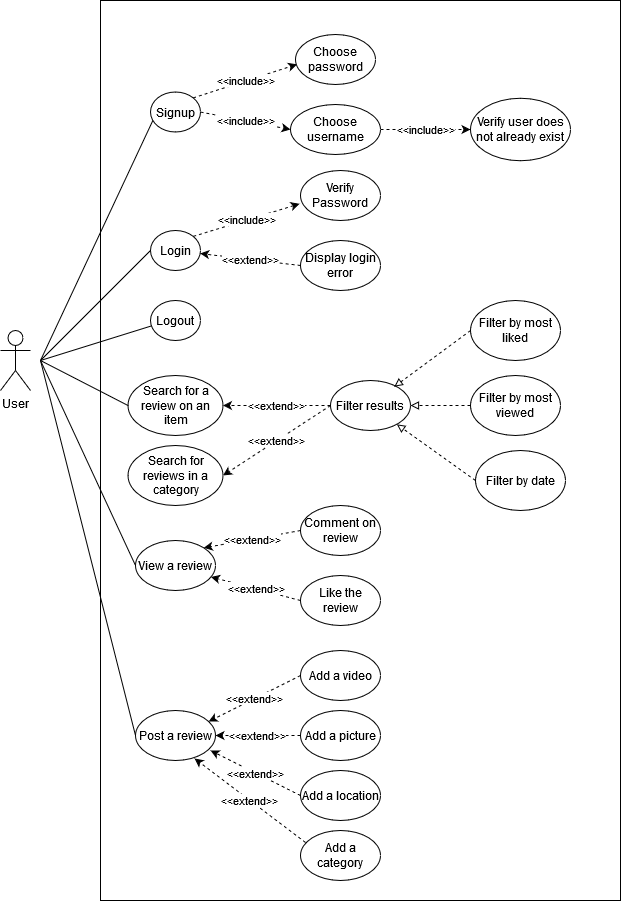
\includegraphics[width=4in]{Figures/Meri Raye Use Case.png}
        \caption{The use case diagram of the application.}
        \label{fig:use-case}
    \end{figure}
\end{center}

\newpage
\justify
\section{Use-Case Descriptions}
% Add use-case descriptions per the given template %

\subsection{Sign-up}
\begin{table}[H]
    \begin{center}
        \begin{tabular}{ |m{6cm}|p{6cm}| } 
           \hline
           \textbf{ID} & 01\\
           \hline
           \textbf{Title} & Sign-up/Register for \textbf{Meri Raye}.\\
           \hline
           \textbf{Description} & A new user is added with a unique username to the Meri Raye application.\\
           \hline
           \textbf{Primary Actor} & An unregistered user.\\
           \hline
           \textbf{Preconditions} & The user being added must not already exist as a member of Meri Raye.\\
           \hline
           \textbf{Postconditions} & A new user is profile is created in the application with a unique username.\\
           \hline
           \textbf{Main Success Scenario} & We first verify that the user registering does not already exist. If he/she doesn't already exist, we create a new user profile with their given credentials (username) and allow them access to Meri Raye.\\
           \hline
           \textbf{Extensions} & An error will occur when the user that is registering is already present as a member of Meri Raye.\\
           \hline
           \textbf{Status} & In progress.\\
           \hline
           \textbf{Priority} & High priority.\\
           \hline
        \end{tabular}
    \end{center}
    \caption{\label{tab:Table 1} Detailed description for $<\textit{sign-up}>$.}
\end{table}

\newpage
\subsection{Log-in}
\begin{table}[H]
    \begin{center}
        \begin{tabular}{ |m{6cm}|p{6cm}| } 
           \hline
           \textbf{ID} & 02\\
           \hline
           \textbf{Title} & Log into \textbf{Meri Raye}.\\
           \hline
           \textbf{Description} & A registered user is attempting to log into the application.\\
           \hline
           \textbf{Primary Actor} & A registered user.\\
           \hline
           \textbf{Preconditions} & The user being added must already exist as a member of Meri Raye.\\
           \hline
           \textbf{Postconditions} & The user is allowed to access the features of the application and their user profile, if he/she correctly inputs their username and password for the log in.\\
           \hline
           \textbf{Main Success Scenario} & We first verify that the user registering already exists. If he/she does already exist, we allow them access to their user profile and to the features of Meri Raye.\\
           \hline
           \textbf{Extensions} & An error will occur when the user that is logging in is not a member of Meri Raye, or they have input either their username or password incorrectly.\\
           \hline
           \textbf{Status} & In progress.\\
           \hline
           \textbf{Priority} & High priority.\\
           \hline
        \end{tabular}
    \end{center}
    \caption{\label{tab:Table 2} Detailed description for $<\textit{log-in}>$.}
\end{table}

\newpage
\subsection{Log-out}
\begin{table}[H]
    \begin{center}
        \begin{tabular}{ |m{6cm}|p{6cm}| } 
           \hline
           \textbf{ID} & 03\\
           \hline
           \textbf{Title} & Log out of \textbf{Meri Raye}.\\
           \hline
           \textbf{Description} & A registered user is attempting to log out of the application.\\
           \hline
           \textbf{Primary Actor} & A registered user.\\
           \hline
           \textbf{Preconditions} & The user who wants to log out must already be logged into the application.\\
           \hline
           \textbf{Postconditions} & The user is logged out of the application and can no longer view his/her user profile or access the features of the application.\\
           \hline
           \textbf{Main Success Scenario} & If the user is already logged into the application, then and only then is he/she allowed to log out of the application. After logging out he/she is returned to the log-in/sign-up screen and can no longer view his/her profile or use the features of the application.\\
           \hline
           \textbf{Extensions} & N/A.\\
           \hline
           \textbf{Status} & In progress.\\
           \hline
           \textbf{Priority} & High priority.\\
           \hline
        \end{tabular}
    \end{center}
    \caption{\label{tab:Table 3} Detailed description for $<\textit{log-out}>$.}
\end{table}

\newpage
\subsection{Search for a review}
\begin{table}[H]
    \begin{center}
        \begin{tabular}{ |m{6cm}|p{6cm}| } 
           \hline
           \textbf{ID} & 04\\
           \hline
           \textbf{Title} & Search for a review on the application.\\
           \hline
           \textbf{Description} & A registered user wants to search for a review on an item or wants to search for reviews in general for a category of his/her choice.\\
           \hline
           \textbf{Primary Actor} & A registered user.\\
           \hline
           \textbf{Preconditions} & The user who wants to search has input a keyword or chosen a category and has pressed the search button.\\
           \hline
           \textbf{Postconditions} & The user is presented with a list of search results according to the keyword he/she has entered or the category he/she has chosen.\\
           \hline
           \textbf{Main Success Scenario} & The user inputs a keyword or chooses a category of items he/she wants reviews on and presses the search button. The system searches for reviews according to the item or category that has been requested. If it finds reviews that match the search criteria, the user is presented with a list of the search results (i.e., reviews).\\
           \hline
           \textbf{Extensions} & An error will occur when the customer presses the search button before he/she has entered a keyword or chosen a category. \newline An error will occur when there are no reviews matching the search criteria of the user, in which case an error message is displayed.\\
           \hline
           \textbf{Status} & In progress.\\
           \hline
           \textbf{Priority} & High priority.\\
           \hline
        \end{tabular}
    \end{center}
    \caption{\label{tab:Table 4} Detailed description for $<\textit{search for a review}>$.}
\end{table}

\newpage
\subsection{Post a review}
\begin{table}[H]
    \begin{center}
        \begin{tabular}{ |m{6cm}|p{6cm}| } 
           \hline
           \textbf{ID} & 05\\
           \hline
           \textbf{Title} & Post a review on the application.\\
           \hline
           \textbf{Description} & A registered user wants to post a review on an item of his/her choice, with the option to add videos and pictures. A location and a category are mandatory with every review that is to be posted on the application.\\
           \hline
           \textbf{Primary Actor} & A registered user.\\
           \hline
           \textbf{Preconditions} & The user who wants to post a review on an item has drafted his/her review, added a location and a category and provided optional additional attachments. The user has then pressed the “post review” button.\\
           \hline
           \textbf{Postconditions} & The user is notified that their review has been successfully posted on the application.\\
           \hline
           \textbf{Main Success Scenario} & The user drafts their whole review on the item of their choice and have added a location and a category for the item they are reviewing (mandatory). They can also, additionally, choose to add a video and/or a photo to their review. Once their draft is complete, they have pressed the “post review” button. Their review is then posted on the application and a notification saying “successfully posted” is displayed to them.\\
           \hline
           \textbf{Extensions} & An error can occur when the customer omits adding either the location or the category in their review, since these are required for a review to be posted on the application.\\
           \hline
           \textbf{Status} & In progress.\\
           \hline
           \textbf{Priority} & High priority.\\
           \hline
        \end{tabular}
    \end{center}
    \caption{\label{tab:Table 5} Detailed description for $<\textit{search for a review}>$.}
\end{table}

\newpage
\subsection{Remove a user}
\begin{table}[H]
    \begin{center}
        \begin{tabular}{ |m{6cm}|p{6cm}| } 
           \hline
           \textbf{ID} & 06\\
           \hline
           \textbf{Title} & Remove a registered user from the application.\\
           \hline
           \textbf{Description} & An admin has the right to remove a registered user from the application at any time provided he/she has violated any of the rules and regulations.\\
           \hline
           \textbf{Primary Actor} & An admin.\\
           \hline
           \textbf{Preconditions} & The user to be removed is a registered user on the application and has violated any of the rules and regulations.\\
           \hline
           \textbf{Postconditions} & The user now no longer exists as a registered user of the application.\\
           \hline
           \textbf{Main Success Scenario} & The admin notices a registered user has violated a rule of the application. The admin therefore removes that user from the application.\\
           \hline
           \textbf{Extensions} & N/A.\\
           \hline
           \textbf{Status} & In progress.\\
           \hline
           \textbf{Priority} & Medium priority.\\
           \hline
        \end{tabular}
    \end{center}
    \caption{\label{tab:Table 6} Detailed description for $<\textit{remove a user}>$.}
\end{table}

\newpage
\subsection{Moderate a review}
\begin{table}[H]
    \begin{center}
        \begin{tabular}{ |m{6cm}|p{6cm}| } 
           \hline
           \textbf{ID} & 07\\
           \hline
           \textbf{Title} & Moderate a review on the application.\\
           \hline
           \textbf{Description} & A admin has to moderate a review on the application that a user has posted. This is to be done for every review that is posted.\\
           \hline
           \textbf{Primary Actor} & An admin.\\
           \hline
           \textbf{Preconditions} & A new review has been posted on the application by a registered user.\\
           \hline
           \textbf{Postconditions} & The review that was being moderated may be removed if it is found to be unethical, otherwise it will remain on the application.\\
           \hline
           \textbf{Main Success Scenario} & The admin moderates a newly posted review and decides on whether it is ethical.\\
           \hline
           \textbf{Extensions} & N/A.\\
           \hline
           \textbf{Status} & In progress.\\
           \hline
           \textbf{Priority} & Medium priority.\\
           \hline
        \end{tabular}
    \end{center}
    \caption{\label{tab:Table 7} Detailed description for $<\textit{moderate for a review}>$.}
\end{table}

\end{document}
